\begin{center}
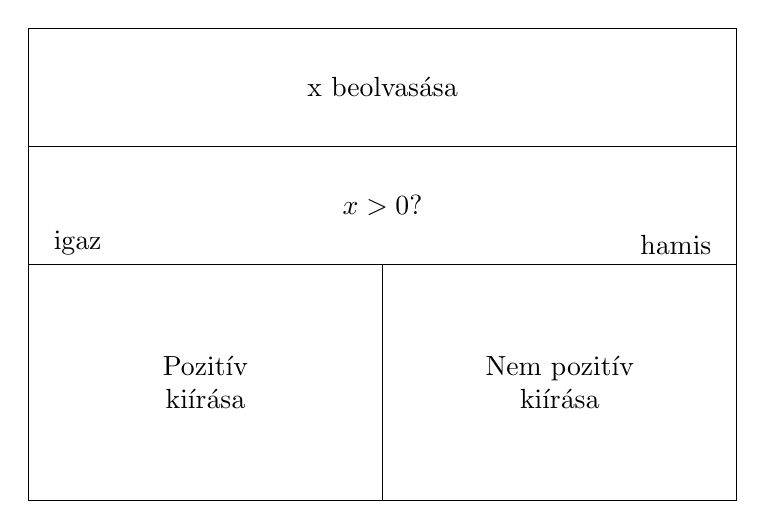
\begin{tikzpicture}[x=1mm,y=1mm]
  \draw (0,0) rectangle (90,60);
  \draw (0,45) -- (90,45);
  \node at (45,52.5) {x beolvasása};
  \draw (0,30) -- (90,30);
  \node at (45,37.5) {$x>0$?};
  \draw (45,0) -- (45,30);
  \node[align=center] at (22.5,15) {Pozitív\\kiírása};
  \node[align=center] at (67.5,15) {Nem pozitív\\kiírása};
  \node[anchor=south west] at (2,30) {igaz};
  \node[anchor=south east] at (88,30) {hamis};
\end{tikzpicture}
\end{center}
